\chapter{}
I woke up, my mind in a fog. I had been dreaming. I usually do not dream, and when I do, it
seems to be a disjointed series of sequences. In the dream, I'd been on a beach with Monique.
She had been sitting on the sand in a blue bikini, with the incoming waves lapping at her bare
feet. Her hair was blowing in the warm wind, and she was smiling at me. Then, we were in a
house, I don't know what it was, but we were both terrified that something outside was trying to
get us. Finally, I'd been with her in a different house. It was a house I'd never been in
before, but somehow, in the dream, I knew it was my house. Even though I was inside, I felt the
wind blowing gently at my hair. Monique was lying in a bed, covered from chin to toes in a full
body plaster cast. Again she was smiling, and asked me for a hug. In the dream, I had told her
``Sure- my Mom likes you.'' As my mind cleared, I recalled the events of the previous day,
wondering if they were part of the dream. Then I realized I could still feel the wind from the
dream in my hair- Monique was laying next to me, she had slipped her right arm under me and
pulled me close to her. With her hand, she was stroking my hair.

``Good Morning,'' she said. \aside{``Great morning, actually,'' she thought to herself.
She had been awake for a while, but she really didn't know how long. She supposed it had been
about thirty minutes, but it could have been longer. She had just been watching Quinn sleep,
thinking about the day before, and her night in the cast. She had slept very well. Despite not
being able to move, the cast had been comfortable. She was truly enjoying this experience; this
wonderful cast, this wonderful man- it was all like a dream, one from which she did not want to
wake.}

``Good morning, yourself. How did you sleep?''

``Very well, actually. I don't think I tossed and turned a bit,'' she said with a smile,
then added ``I'm glad you're awake- I really need to pee.''

I got up, stretched, and pulled the wheelchair back close to the bed. I picked her up, and
set her into the chair. I wheeled her to the bathroom. (The light didn't work, which didn't
surprise me) When she was done, I helped her get the shorts pulled back up (with my head turned)
and got her back into the chair. As I did so, she said ``I guess a shower is out of the
question.''

``Yes, I don't think you'll be doing that.'' I turned on the faucet in the sink, and found
that there was still water pressure. That gave me an idea.

``You can have a sponge bath if you want.''

``Ah, my guardian angel comes through for me again. I'm such a lucky girl.''

``Lucky will be if the water is warm. The water heater is electric, and has been off for
almost 24 hours. Let's hope that what's in the tank has held its heat.'' I went to the casting
room, and got my bucket. I dumped it down the tub, and rinsed it with cold water. I then turned
on the hot water tap, and was pleased to find that the water, while a long way from hot, was not
ice cold. I grabbed a bar of soap, a washcloth and a towel, and placed them on her lap. I
wheeled her into the hospital room, and took the items and set them on the bed.

``This is nice,'' she started, ``but I can't do much with only one arm. Would you help
me?''

I was uncomfortable with the idea, but since she was my responsibility, I couldn't easily
say no. I took the bucket and used the washcloth to wet her face. She gasped slightly at the
cool water.

``I'm sorry about that- It's not very warm,'' I said.

``It's OK, just a little bit colder than what I expected.''

\begin{thought}
Yes, it certainly WAS okay. Monique could almost not believe she was having yet another
highly intense experience with Quinn. First, he gently washer her face and neck. Then, she
watched as he washed her foot, then up her leg, to mid thigh. He wiped off the soap with the
washcloth, and then dried her with the towel. He then washed her arm. His hands working over her
body was almost as wonderful as when they were making a cast.
\end{thought}

When I was finished with her arm, I told her that she'd have to do her private areas
herself. I helped her pull the shorts down (again with my head turned) and left the room,
telling her that I was going to take a shower, and to be careful to keep the cast as dry as
possible. I ran upstairs, grabbed fresh clothes, and went back downstairs to shower there. I
usually showered in the upstairs bath, but I wanted to be close, in case she needed me.

The shower was cold. No, the shower was frigid. Still, once it was done, I felt better. I
brushed my teeth quickly, and when I returned to the hospital room, Monique was sitting with the
towel on her lap.

``I heard the distinct sound of teeth being brushed. I'm jealous.''

I felt a bit on the spot. ``I'm sorry, Monique, I don't have a spare toothbrush.'' At that
point, I had an idea. There was a small grocery store a few blocks over. It might not be open,
but maybe it was worth a try.

``Monique, there's a store in easy walking distance. If you want, I could go and see if
they're open. If they are, I can grab you a toothbrush and anything else you want.''

Monique didn't really want him to leave, but she really felt nasty with her morning breath.
``That would be great; maybe you could pick up some breakfast, too.''

I said goodbye, and headed out the door to the market. The Saturday was as beautiful as the
Friday before had been ugly. The late morning sun shone brightly, a few fluffy clouds drifted
lazily by, and a light breeze blew. As I walked, I passed a lot of houses that were damaged by
the storm. Many of the people were outside, cutting downed trees and limbs with chainsaws.
Others were picking up debris, and some were covering damaged roofs with plastic sheet. As I
neared the market, I remembered that there was also a hardware store on the same corner.

Hacksaw blades. Tin snips. Monique out of the cast! I walked the last block quickly, almost
running. As I reached the corner, my happiness faded quickly, as I saw both the grocery and the
hardware store were dark. Though they were not damaged, signs on the door announced that they
were closed until the power was restored to them. I turned, dejected, and just stood there for a
minute, not knowing what to do next.

As I stood, gathering my thoughts, I noticed a little further up the block was a
convenience store, and there was a car parked at one of the pumps, with someone pumping gas into
a green SUV. I walked to the store, and went inside. It was a pretty well stocked store, and I
quickly found a toothbrush. I hadn't thought of it before, but I saw a hairbrush, and thought
she might like to brush her hair. Thinking about the batteries in the boom box, I picked up a
couple of spare sets of batteries. I also got a half dozen bagels, a gallon of milk, more
cigarettes, and, as an afterthought, I got two large cups of hot coffee.

When I returned home, Monique was waiting for me in the parlor. She'd managed to wheel
herself in there, and had turned on the battery operated stereo.

``Sorry it took so long, the store was closed, but there was a gas station open close
by,'' I said, handing her the toothbrush. ``And, I thought you might like this,'' I said,
handing her the hairbrush.

``Thank you. You don't know how much I appreciate this'' she said, as I wheeled her into
the bathroom, and turned her to be close to the sink with her right arm.

``Monique, you'll never know how much I appreciate your being so calm and understanding
through all of this,'' I answered.

``Quinn,'' she sighed. ``I don't know how many times I need to tell you this, but the
storm was not your fault. I wouldn't blame you if I was in misery right now. But, I'm NOT in
misery. No, I don't want to be like this forever, but we both know that's not the case. You made
me a great dinner last night; we shared some good music, and had fun playing chess. The cast is
not uncomfortable, and I slept well. All in all, this has been the best date I've had in a long
time,'' she said with a smile.

A date. She described it as a date. I didn't know how to respond to that, other than to
lighten the tone a bit.

``Yes, I sure know how to show a lady a great time, huh?'' I said sarcastically.

``As a matter of fact, I did have a great time. Now, I don't mean to be rude, but I'd like
to brush my teeth in private. It's not ladylike to spit in front of a man.''

I couldn't help but chuckle to myself as I walked out and pulled the door shut behind me.

While Monique was brushing her teeth, I got out the bagels, and set them on the table with
the coffee. From outside, the familiar noise of a chainsaw started, much louder than I was used
to hearing. I looked out the back door to see two men working on the tree that lay across the
remains of my truck.

When Monique was finished, she called out to me, and I moved her to the kitchen. We ate the
bagels as I told her about what I'd seen on my trip to the store. I told her about my idea of
finding something at the hardware store to cut the cast off. As I mentioned my ideas to her, she
had an odd look in her eyes. I was too far past trying to attach some meaning to her reaction-
It seemed to be disappointment, but disappointment at what? Was it because I'd failed in my
mission? Or could it have been because she wanted to stay in the cast longer? At that point, I
really had no idea. She was in a huge cast, and didn't seem to mind, so I had to accept that it
was possible that she might be enjoying herself. It was far fetched, but she'd given clues that
she might like wearing the cast. Then again, she could easily not like the cast, but just be
calm enough to accept it until getting her free was possible. Then again, it could al be a
masterfully executed attempt to appear as though she enjoyed it, to maybe get to the man with
the money. At this point, I wanted to doubt that, but I couldn't completely shake the thought,
either.

We finished eating, and went to the living room to sit in the sunlight. Monique broke the
silence.

``Quinn, can you help me out of this chair? My butt is getting sore from sitting for so
long. I'd like to change position if I can.''

I thought for a moment about how best to change her position.

``How about if we put you on the couch- leaning farther back?'' I asked.

She nodded her consent, and I picked her up from the chair, and set her on the couch. I
got some pillows from the hospital room, and propped them under her leg to raise it enough to
move the center of her weight further back. She was leaned back further, and looked more
comfortable. I could only apologize once more for her predicament, and she reassured me once
more.

The sounds of the chainsaw had stopped, and the men were loading the wood from the cut
tree into their truck. They had gotten quite a bit loaded already, and were making quick work of
the remains.

``Monique, they've almost gotten the truck uncovered. The inverter may be undamaged. I'm
going to go check.''

``Okay. I'll be fine,'' she replied, with that same almost disappointed look to her eyes
again.

\begin{thought}
When Quinn went outside, Monique thought to herself: ``I've got to tell him. I've got to
tell him everything. It's just not fair for him to be so desperate to find a way to cut me out
of this cast when I'm really not ready to be out of it. He's thinking that I'm miserable, and
I'm enjoying myself.'' She also knew that she had to tell him about her feelings for him. At
breakfast, she had mostly just thought about the night before, sleeping next to him, enjoying
his closeness. She couldn't keep hiding what she was feeling, even though she thought she was
doing a poor job at hiding it. She thought her actions made her feelings totally transparent.
She had to get the nerve to tell him.
\end{thought}

In the backyard, I took a look at the truck, and was not encouraged. The cab had been
totally flattened. I hadn't noticed with the tree on it, but the entire truck had been so
crushed that the frame had bent in the middle. The roof of the cab was now pushed against the
seat, and the inverter had been sitting on the seat.

I went to the garage, and got the tire iron from the Mustang. I went back, and tried to
pry open the driver's side door of the truck. I did not have enough leverage to pry it open, so
I tried the passenger door. It gave a little bit, so I kept working at it. I finally got it to
open enough to poke my head inside. The floorboard was strewn with broken glass and pieces of
tan plastic from the interior of the truck. Also scattered were some small pieces of black
plastic- pieces of the inverter's plastic cover. My heart sank. This had been wasted effort- the
inverter had been smashed to bits.

I took the tire iron back to the garage, and looked around for anything that I might use on
the cast- nothing. I prayed for the power company to return quickly. If they weren't back soon,
I'd go try the hardware store again. As I walked back to the house, I had another idea.

I went back inside, told Monique about the inverter, and found my phone book. If I could
just get the truck moved out of the way, I could load her in the Mustang, and take her to a
motel with power. We could have her out quickly.

I called every towing service in the phone book. Most of the numbers came back as out of
service. The few times I actually got through, I was told differing times that they could get
someone there, and the best estimate was Monday. The storm had the towing services all busy with
removing damaged vehicles, and I would have to wait my turn. I hung up the phone, and turned to
Monique.

``I'm sorry, but I'm out of ideas. Unless the hardware store opens, I don't have any way
to get the cast off until the power comes back on.''

``So we'll wait,'' she replied.

``I can't believe that you're so calm about this!''

``Quinn, did you even listen to me earlier?'' she said, not in an accusing tone. ``I'm OK
with this. I'm not uncomfortable in the cast, I swear. I'll be alright.'' She paused a moment,
as if searching for words, then said ``I'll be fine until the power comes back on, if you'll
just quit being so stressed about it, Okay?''

``Okay,'' I answered.

\begin{thought}
``You were so close, how could you chicken out?'' Monique asked herself. ``You need to
tell him the truth, all of it.'' She had almost told Quinn about liking the cast when she'd
paused, but just couldn't bring herself to. She knew that she had to tell him, though. She had
to tell him soon. Maybe she could soften him up a bit, and feel him out.
\end{thought}

Monique used her right arm and leg to turn herself on the couch, so that she was facing
forward, and sitting upright again.

``Come here and sit,'' she said, pointing to the floor in front of her. I sat down facing
her, and she instructed me to turn around. When I did, she used her right hand to massage my
shoulders and neck. She was really good, especially since she was only using one hand. I hadn't
realized it until then, but my neck was very knotted up. I thought for a moment about exactly
where I was: at my left was the casted leg of a beautiful woman who was using her free hand to
massage my neck and shoulders. It was quite a moment for me.

``How's this?'' she asked.

``It feels great. Thank you.''

``You're welcome. I wish I'd thought of this earlier, Quinn. You're seriously tied up in
knots.''

\begin{thought}
``And I'm tied up in knots inside,'' she thought to herself. She was thrilled at touching
him, helping him. She was torn inside; she felt sorry for him, and just wanted him to relax and
enjoy the moment as she was, yet, she couldn't deny that it was nice to know he cared enough to
be so concerned for her. She had to tell him. She had to tell him now, but she just couldn't
bring herself to do it. She decided to change the subject.
\end{thought}

``Let's just turn on some music, and enjoy the day. It's really beautiful outside,'' she
said.

During the afternoon, we listened to CD's, played chess, and talked. I made a sketch of
her sitting in the wheelchair. I checked several times to see if the power was back on, but it
was not. I made us sandwiches for lunch, and it was while we ate, that I found myself actually
enjoying the situation. I was with a beautiful woman in a huge cast. She was dependent on me for
everything from food to the restroom, and she seemed not to mind. She'd been in the cast for
well over 24 hours, now, and it didn't seem to be bothering her one bit. It had taken me longer
to get to the point, but I was now enjoying it, too. Before we knew it, the afternoon had faded
into a beautiful sunset, and the sound of chainsaws began to fade away as people stopped cleanup
work for the day.

``Quinn,'' Monique said, ``Let's go sit outside. It's so nice outside, and I've been
indoors all day.''

``Let me go get something, and I'll be right back.'' I went upstairs, remembering how
she'd been a bit cold last night when we were outside. I grabbed a sweatshirt, and went back to
her.

``Maybe you'd prefer this to wrapping up in a blanket,'' I said as I helped her into the
sweatshirt.

``It will be a lot easier to eat this way. Thanks.''

In the sweatshirt and shorts, she didn't look quite as helpless as she did when the entire
cast was visible. Of course, she was every bit as immobilized, but the cast was only visible at
her hand and leg. At a quick glance, someone might have thought she just had a broken leg, and
some sort or wrist or hand injury. Of course, any further looks would have revealed the arm not
to move, and the distinct line of the cast where it crossed her upper chest to her shoulder
showed through the shirt. I picked her up and set her in the wheelchair, and took her outside. I
got the candles, and a couple of beers, and we sat on the deck. We enjoyed the evening in
silence for a few minutes, until Monique broke it.

``Quinn, what I'm about to say may sound strange.''

The comment struck me as amusing. ``Monique,'' I started,'' we're sitting outside a damaged
house, near a devastated neighborhood. You're completely healthy, yet you're wearing a body cast
that I put on you to satisfy someone's strange sexual fetish. Now- you were saying something
about strange?!''

She laughed at my comment. ``Ok, you win- we are already off of the beaten path. But,
there's something I wanted to say to you.''

I wasn't sure what to expect, but since this sounded somewhat important to her, I turned
to look her in the eye.

``Quinn… I'm having a really good time. I really enjoy being with you.''

I didn't know what to say. I'd had a million conflicting feelings about Monique since I'd
met her, but until now, I'd never really considered that she might have romantic feelings for
me. I was at a loss for words. She seemed to sense this, and went on.

``When I made the remark about this being the best date I'd had in a long time, I was only
halfway joking. I hope it doesn't make you feel uncomfortable, but I've wanted to spend more
time with you for a while, now.''

``Monique, you're not exactly a bad person to spend time with, yourself,'' I said. This
wasn't a lie. She had a lot of good qualities: she was a good conversationalist; she had good
taste in books and music (or at least taste similar to my own), she was smart, and of course,
she was very easy to look at.

I thought for a moment, and added ``Honestly, it's been the best date in a long time for
me, too.''

She held out her hand to me, and I took it in mine. It felt good. Somewhere, in the back
of my mind, a voice was reminding me of the bad opinions I'd had about her, but it wasn't loud
enough to distract me from the warmth of her hand in mine. She pulled me closer, looking me in
the eye. She didn't say a word, but the look in her eye was as clear as day. We melted into a
long, gentle kiss. Although probably not forever, the voices in my head shut up.

After the kiss, I again didn't know quite what to say. The best I could come up with was
``Are you hungry?''

A lot of women would have been bothered by the subject change, but Monique seemed to
appreciate the relaxing of the tension. ``Yes, I am. What's for dinner, Chef Quinn?''

``You'll see,'' I said, turning to go to the kitchen. I'd been thinking about what to make
for dinner if power had not been restored, and it looked to be a good thing that I had. Using
the flashlight, I took a pot, and filled it with water. I took the pot out, set it on the grill,
and turned the grill on. As I waited for the water to boil, I opened a pre-measured pasta salad
mix, and combined the ingredients for the dressing. I then went to the freezer, and took out
some fresh crappie fillets that I'd had the good fortune to find at a local market a few days
ago.

I went back outside, and checked on the water. It was boiling, so I dumped in the pasta,
and sat down with Monique while it cooked. I took my cigarettes, lit one for myself, and offered
her one. She nodded, so I took one out, and lit it for her.

\begin{thought}
``Go ahead- tell him the rest,'' She thought to herself. The first part had gone well, now
you owe him the rest of the truth. But- the first part had gone SO well, she was afraid to admit
that she enjoyed the casts, too.
\end{thought}

``You're quiet,'' she said.

``I'm sorry, it's just that the last day and a half has been…. Intense.''

``Yes it has. We had some serious lows, and some good moments, too. We also had one moment
that I thought was pretty great,'' she said, smiling.

``It was great,'' I said.

``I hope you don't think that my kissing you was because of what happened yesterday. I've
wanted to do that for a while, now.''

``I believe you, but it did take me by surprise.''

She laughed. ``And I thought I was totally transparent about it.''

``Maybe you were,'' I commented. ``I've never been good at picking up the subtle hints.''
I stood up. ``And now, I need to continue with our dinner.''

I went to the grill, got the pot of boiling water and pasta, and took it into the kitchen.
I drained the pasta, and mixed it in with the dressing. I then took the fish and a skillet
outside, and sautéed the crappie with butter. Monique watched me cooking, not saying anything.
When it was fully cooked, I took it back inside. I put the fish on plates, added some pasta
salad, and took them out to the deck. I placed one plate in front of her, and the other on my
side of the table.

She sniffed the plate. ``This smells delicious,'' she said.

``One more thing- something to drink. I'll be right back.''

I went to the kitchen, and got two glasses, and a bottle of Sauvignon Blanc. I took them
outside. I poured some for each of us, and sat down.

Dinner was pretty good, if I do say so myself. Monique complimented me on it, also. When
we were done, we sat there in the moonlight, sipping our wine.

\begin{thought}
Monique knew it was time. She was sure that the wine had added to her courage, and she was
glad for it. ``OK,'' she said to herself,'' here goes.''
\end{thought}

``Quinn, I have something else to tell you.''

``What's that?'' I asked, not expecting what I heard next.

``Monday, when you saw me at the bookstore, and I had my ankle wrapped up- I wasn't hurt.
I didn't sprain my ankle.''

I had wondered about her. I had almost thought that she maybe liked casts, but thought I
was either imagining it, or that she was pretending in an attempt to get at the money behind the
operation. That might still be true, but at this point, I was hoping that it wasn't.

``What?'' I asked.

``I didn't sprain my ankle. I wasn't hurt at all,'' she said. ``I am sorry that I lied to
you, but I wasn't sure you'd understand.''

Oh, I was thinking maybe I DID understand. I was hoping I understood, but I was still
cautious.

``Understand what?'' I asked.

``Quinn,'' she asked, ``how much do you know about people's desires when it comes to the
whole casting thing?''

``I know some.''

She looked off into the distance. ``Well, there are a lot of people like your boss, who
enjoy seeing other people casted. It's a sexual excitement for them,'' she said.

``Yes,'' I replied. ``I knew that.''

She went on. ``There are others who like to wear casts. Some just like the feel of them;
some people are turned on by wearing them. Some people like going out in public and drawing
attention, and some like being taken care of in private while wearing casts.''

``I knew about that, too.''

``Quinn, I'm not just tolerating this cast. I like it.'' \aside{There, it was out, and
there was no calling it back, now.}

``You like wearing the cast?'' I asked. ``Can I ask which of the reasons is why you enjoy
it?''

``All of the ones I mentioned and one other. I love the feel of your hands on me through
the plaster or fiberglass as you are making the casts. From the first casts we did, I knew there
was something about it I liked. For a while, I wasn't sure if it was you or the casts that made
me feel that way.'' She stopped and turned her head to look me in the eye. ``I realized a couple
of weeks ago that it is both. When we went publicking with me in the long leg cast (I noticed
she was using correct caster terminology) I had such a great time that I knew that it was being
with you AND being in the cast that I was enjoying. Then, after last week, I went to the drug
store, bought an ACE bandage and some crutches, and faked a sprained ankle to get in a bit more
publicking. Do you think I'm weird?''

``Yes, you're definitely weird,'' I answered. ``But it's not bad weird,'' I added with a
smile.

``Quinn, when I kissed you, I meant it. I really did. I was attracted to you from the
first time I met you, and it's only gotten stronger since.''

This was almost surreal. I felt almost as if I were in a dream. I wanted to take what she'd
said at face value, but my initial impressions of her were surfacing in my mind. I didn't
necessarily believe them anymore, but I couldn't dismiss them, either. I thought for a few
moments about how to approach it, and decided that straight on would be best.

``Monique, you were almost $\ldots$ bitchy when I first met you. Please understand I'm not
picking at you, I'm just telling you what's in my head.''

She lowered her head ``I know I was a bitch at first. I've been hurt in relationships. I'm
not crying about it, just explaining. I've cared seriously about guys, only to find out that
they were only interested in one thing. I'm sure every woman has dealt with that, I just don't
deal with it well. It's almost easier to be cold and distant to just keep people away than to
open up to them and get my heart stomped on.''

I could certainly relate to feeling a need to conceal one's true self, but I had to press
her a bit further.

``You also gave me the impression when I first met you that you were only interested in
money,'' I said.

\begin{thought}
That comment stung Monique. She had never been materialistic. She'd always had to get by on
very little, and be happy with it. She'd always been satisfied without a lot of luxuries and
nice possessions, but she had been in a bad situation when she'd met Quinn, and she supposed
that it had shown through.
\end{thought}

``At that time I WAS only interested in money,'' she said honestly. ``I was seriously
worried about being able to stay in school. I was barely able to keep a roof over my head, and
had no idea how to pay next year's tuition. Between waitressing, and modeling for you, I've
actually been able to get my car fixed, and bank a significant amount of money, too. I've been a
lot happier since that problem has been solved.'' She sounded a bit defensive as she explained
it.

``I wasn't accusing you, Monique. This weekend has been everything but what I'd expected
it to be. You were just very honest with me, and I wanted to be honest with you.''

``I understand,'' she said, ``but it does sound a bit cynical.''

I realized she was right- it WAS cynical. Of course, she didn't know exactly where I was
coming from. I needed to tell her, but I just couldn't bring myself to do it just yet. Maybe it
was everything that had happened over the last 36 hours, or maybe it was just that I wanted to
test her a bit further. I wasn't sure which, but I decided to put a slightly different spin to
it.

``Monique, it doesn't just sound cynical, it IS cynical. There was one woman who I casted
in the past that gave me a distinct impression that she was trying to get past me- to the
wealthy man behind it all.'' I hated the deception in what I said, even though it was all
technically true.

Monique looked disgusted and nodded. ``I know that there are a lot of women out there like
that,'' She said. ``I've known a lot of women who'd take money over love any time. I never could
understand them. It seems so cheap that they would accept that as what they wanted their life to
be. Besides, I can't stand the way rich people act.'' She paused for a minute, and asked me to
come closer. She pulled me close to her face and said ``What I'm feeling for you is real. Even
in our limited contact, you've shown me things about yourself that I like- things that I like a
lot. I'm not interested in the man with the money, I'm interested in you.'' At that, she pulled
me into another kiss. We smiled at each other, and then I pulled my chair up next to the
wheelchair. We sat next to each other with our arms around one another for a while, just
enjoying the evening and each other's company in silence.

\begin{thought}
Monique enjoyed Quinn holding her. She had been a little hurt by some of the things he'd
said, but the more she thought about it, the more she saw why he had thought them. Besides, it
seems that it hasn't hurt her chances with him. It looked like she was going to have a chance to
show her real self to him. She knew it was an extreme chance to take. She knew she could be hurt
worse than ever before by Quinn, but she wasn't very worried. She really felt that Quinn was
genuine and true. She felt that whatever happened between them, she would make a friend that she
could keep forever.
\end{thought}

As we sat, watching the moon drop from the sky, I was lost in my thoughts, and in the
moment. I was holding a beautiful woman in my arms. She was wearing an enormous cast, and she
was enjoying wearing it. She also had serious feelings for me. Life was good. I was also
pondering the facts I hadn't shared with her, such as the fact that I was the man behind all of
this. I wanted to tell her, and I knew I needed to. Between what she'd said about not liking the
actions of wealthy people, and nagging concerns about her that I had, I decided to wait to tell
her. I wouldn't deceive her long, but I wanted to prove myself to her, and also to prove her
intentions to myself.

I heard soft snoring, and turned my head to look at the head lying on my shoulder. Monique
looked very beautiful in the dim fading moonlight. She looked so peaceful, and seemed to have a
contented look on her face. I got up gently, and wheeled her to the hospital room. She woke up
as I picked her up and laid her on the bed.

``Please snuggle with me,'' she said groggily. I was glad she'd asked. I slipped in close
to her, and pulled a blanket over us. She laid her head back on my shoulder, and was quickly
asleep again.

I pondered what was happening, what was starting. I wasn't sure, but it felt good for the
time being, and as long as it felt good, I decided to follow it wherever it led.

I didn't know when I drifted off to sleep, but when I woke up, I felt fantastic. I had
slept very well. The sun was peeking through the windows. I looked next to me, and Monique was
right where she'd fallen asleep. (Of course, tossing and turning would have been a little
difficult) In my sleep clouded mind, I heard a strange whirring noise. As my head cleared up, I
recalled the events of last night. It was all real, I hadn't dreamed it. The noise didn't go
away as my thoughts became more coherent. It seemed to be coming from the other room. Then I
recognized it- it was the ceiling fan in the bathroom- the power was back on!

I got up and went to check, and sure enough, I'd left the switch on in the bathroom. When
the power had come back on, the fan and light had started up. I wondered what time it was. I
checked my watch, it was 9:30. It was strange the difference that 24 hours could make.
Yesterday, I'd have started cutting on the cast before she'd even had a chance to wake up.
Today, things were very different. I decided to see if I could sneak back into bed without
waking her up. I knew I needed to get her out as soon as possible, but I decided to get one last
embrace with her in the cast if I could. I turned off the light and the fan quit with it. I
snuck back into the bedroom, and climbed back into bed with her. She stirred only enough to wrap
her free arm back around me. Soon, we were both asleep again.

When I woke up again, Monique was awake, watching me. In other circumstances, that would
have made me uneasy, but not this time.

``Good Morning,'' she said with a smile.

``Good morning to you, too. How does a nice, long shower sound?''

``It sounds great, but don't tease me'', she replied.

``I'm not teasing, the power is back on.''

``I'm not sure how to feel about that,'' she said. ``Part of me is ready to be out, and
part of me doesn't want this to end.''

``Let's get you out of that cast. I promise you can have more casts later.''

``OK. The shower really does sound good. But I need to pee, first.''

``Do you want to take care of that before the cast comes off?'' I asked.

``Yes, I'm not sure I can hold it.''

I picked her up from the bed, and placed her into the wheelchair. I helped her use the
bathroom, and when she was done, I went back and got her. I wheeled her into the casting room,
and put her on the table. Monique was tall, and with the heavy cast, she should have been very
heavy. She never seemed to be that difficult to lift.

I took my sweatshirt off of her. I took a towel, and placed it over her lap, and reached
underneath to pull off the shorts.

``With everything that has happened, you're still not comfortable seeing me naked?'' She
asked.

I stopped what I was doing, and looked her in the eye. ``Monique, this has been an intense
weekend. I like you, Monique. I like you a lot. I don't know where this whole thing between us
will go, but I plan to enjoy finding out.'' I went on. ``If or when we get to the point where it
is right, I'll enjoy looking at your naked body. Until it's the right time, though, I'm going to
respect your modesty. Do you understand what I mean?''

\begin{thought}
Monique couldn't believe she was hearing this. I think he means he doesn't want to see me
naked until he's sure he loves me. I've never known anyone like this. I didn't think men with
this kind of honor still existed.
\end{thought}

``Yes, I understand, Quinn. I appreciate it, too,'' she said, pulling me into a kiss.

``Thanks. Some women do not appreciate someone who treats them with honor and respect.
Now, let's set you free.''

She nodded silently, and I plugged in the cast saw, and started to work. I began by cutting
the cast along the top of her arm from the neck to the fingers. I then went to her right side,
and cut the cast from her armpit to her hip. I was hoping to get this cast off in two pieces. I
was hoping to get it off fairly intact. It would really be nice in my collection. I knew I'd
have to get rid of the collection sooner or later, but I wanted to save this one for a while.

The next cut was delicate. I started at the inside of her left thigh. She giggled a bit as
the vibrations from the saw tickled her. I made sure the towel stayed in place, even though I
really wanted a peek. I cut down the inside of her left leg, and then turned to the final cut.
The final cut went from the toes on her left foot all the way up the leg, past the hip, up to
the armpit, and down the arm to the hand. I pried the cast apart with my hands slightly, and
then went to cutting through the stockinette and padding. I now had the cast completely in two
pieces.

``Ok, Monique, I'm going to pull off the top part of the cast. You can use the towel to
cover yourself up with.''

``Sounds good to me, doctor.'' She said with a smile.

I pulled the top of the cast off. She was a little bit slow with the towel, and I got a
very brief, very nice look at her. The image would stick in my head for a very, very long time.
Her body was perfectly shaped, and the stockinette had imprinted its pattern on her beautiful
tanned skin. I set the fiberglass aside, and turned to face her.

``Monique, you're going to be very stiff. Let's take this slow. Start by bringing your arm
out of the cast. She pulled her arm out and leaned slightly forward. She moved the arm around
slowly, as she held the towel up with her right hand.

``Wow, I really AM stiff.'' She said.

``It's going to take some time to wear off,'' I told her. ``Ok, let's get you completely
free. Lean to your right, and I'll pull the rest of the cast off.''

She switched to her left hand to hold up the towel, and set her right hand on the bed as
she leaned over. When her butt was off of the cast, I pushed it back slightly, and then pulled
it away to her left. I then helped her to sit back up straight.

``Are you alright?'' I asked.

``Yes, just very stiff.'' She replied. ``Help me to stretch a little bit.''

I helped her to work out the stiffness in her muscles that had essentially had the entire
weekend off. She looked breathtaking, with her imprinted skin mostly exposed, save for the
towel. I helped her stretch out while she sat, until she said she was ready to try standing. She
wrapped the towel around herself, and held out her hands to me. I took her hands, and pulled her
to her feet. She was wobbly and slow, but she was able to walk around. She leaned on me as we
walked around the room, reviving her unused muscles.

After a few minutes, I could see that she had recovered quite a bit from the
immobilization.

``Are you ready for the shower, yet?'' I asked.

``I'm thinking a nice long hot bath would be perfect,'' she said.

``OK, I'll leave you to it,'' I told her. ``Will you be alright?''

``I think so. I never expected to be so stiff!''

``That's to be expected when you're immobilized that much for that long,'' I said.

``Quinn, it was worth it. I really had fun in the cast. Part of me misses it. I'm not sure
if that makes sense or not, but that's how I feel.''

``I think I understand, Monique. Go ahead and get your bath. I'm going to go set up
another surprise for you. I'll be back inside within a few minutes. If you need me, just yell,
and I'll come running.''

``I'll be fine. I promise,'' she said as I walked out of the bathroom.

\begin{thought}
Monique went to the tub and sat on the side of it. She let the towel fall to the floor,
and turned on the water. She adjusted it until it was nice and hot, and then slowly lowered
herself from the side of the tub into the water. It felt fantastic. She adjusted the water to be
a little hotter, and when the tub was full, she turned it off. She sat there, soaking, and
thinking. She wondered how much Quinn understood her love of wearing casts. She still had doubts
that he wasn't interested in casts, too. She wasn't sure, but he had given little signals that
he was into this fetish, too. The hot water loosened up her muscles, and the longer she sat, the
better she felt. In addition to the effect the heat and water was having on her muscles, just
getting clean felt great to her, too.
\end{thought}

While Monique took her bath, I went out to the garage. I still had to get her home.
Driving her was impossible, as the truck was still in front of the garage, and wouldn't be moved
until sometime tomorrow. I couldn't get the Mustang out, but there was enough room to get the
Harley out. Monique had mentioned that she liked bikes to me before, and it was the only option
besides walking, which I didn't think she'd be quite ready for. I opened the garage door, and
pushed the heavy softail out through the door. There wasn't much room to spare, but I got it
out, and didn't have to start it. I pushed the bike around to the side of the garage, so she
wouldn't see it unless she actually went outside.

I went back inside, and from the bathroom, I heard the sound of water draining from the
tub. I wasn't surprised when I heard the shower kick on for a few minutes after that. Shortly
after the shower stopped, the bathroom door opened, and Monique poked her head out.

``Quinn!''

I walked to the door. Her hair was wet, and brushed out straight. ``What do you need?'' I
asked.

``A hair dryer and my clothes, or what's left of them.'' She answered.

``Monique, I don't have a hair dryer. Let me get your clothes, though.''

I went to the casting room, and picked up her shorts, bra, top and sandals. I took them to
her, and she thanked me as she closed the door. A few minutes later, she emerged. She was moving
very well, now. Time and the bathing had removed the pattern of the stockinette from her skin.

``You look good,'' I told her.

``Thanks, I feel like a bad girl- I'm not wearing any panties,'' she said with a smile.

I chuckled a bit. ``Would you like to go get something to eat?''

``Yes, I'm starving,'' she said.

``Let me get a quick shower, and we'll go.''

``Exactly how are we going to go?'' she asked.

``You'll see.'' I told her with a smile of my own.

I went upstairs, took a quick shower, and dressed myself in fresh clothes. When I came back
downstairs, Monique was at the kitchen sink, washing the dishes from our meals.

``You didn't have to do that.'' I told her. ``You were the guest!''

``You did all of the preparation. You were a wonderful waiter. You even cut my meat for
me. This is the least I can do.''

``Ok, let me take care of one more thing, and we'll get going.'' I picked up my cell
phone, and punched in the number of the cell phone. It rang a few times, and when my voice mail
picked up, I started talking to it, as though I were actually talking to a real person. ``Yes,
sir, it's Quinn….. We're okay, but we had an interesting problem, here…..Yes, we were in the
middle of a casting session when the storm hit…. Monique was in a fantastic white fiberglass
shoulder and hip spica, and the storm knocked out our power. I just got her out of the cast an
hour or so ago….. Yes, she spent two days in the cast…. She did OK, actually…Yes, I told her we
would, but I wanted to check with you as to how much…. I think that's fair, too. I don't think
she'll have any problem with that…. OK, I'll do that…..yes, I'll send you the pictures and
sketches tonight. I think you'll like them….. Ok, will do. Bye.''

``Monique looked at me. ``The boss?''

``Yes. I wanted to see how much he wanted to pay for the weekend. Hang on, let me get your
money, and we'll get going.''

``Okay,'' she replied.

On my way upstairs, I noticed she had not asked how much. I realized it was really silly
to be looking at the little things to disprove my original impressions of her. She cared for me.
I knew that wasn't an act. At least I was pretty sure. I felt something for her, but it wasn't
definable at the moment. I needed to trust her. I counted out the money, put it in an envelope,
and took it back downstairs, and handed it to Monique.

Her brow furrowed when I handed her the envelope, and when she looked inside, her jaw
dropped.

``Quinn, how much money IS this?''

``Three thousand. He wanted you to be well compensated for the dire circumstance, and the
unexpected stay in the cast.''

``Quinn, that's beyond well compensated. I really feel weird taking this, since I enjoyed
the whole weekend so much,'' she said.

``Just take it. I learned a long time ago to just take it. I'm getting combat pay for the
weekend, too.''

``Okay,'' she shrugged. ``But I really did enjoy it.''

I smiled at her. ``Monique, I enjoyed it, too.'' At that she hugged me. I held her for a
few moments, and then said. ``Are you ready to get something to eat?''

``Starved.''

``Let's go,'' I said, heading to the back door. I opened the door, and held it open for
her, and followed her out. I took her hand, and led her around to the side of the garage. When
she saw the bike, her eyes lit up.

``Care to travel by scooter?'' I asked.

``Yes, sir!''

I got on the bike, and started it. Monique got on behind me, and I put it in gear, and we
rumbled off down the road. It was a beautiful day for a ride, and with Monique behind me, with
her legs wrapped around me, it was even better. We cruised through town slowly, examining damage
whenever we saw it. The town had been hit hard by the storms. We passed a crew mulching downed
tree limbs into a large pile. We got on the highway, and actually headed across the river into
Indiana before we finally stopped at a truck stop to eat. Over lunch, we talked and laughed.
Afterwards, we rode back to town, enjoying the day and the wind in our faces. I decided to go
ahead and take Monique home. I had taken her home once before, and I remembered the way. As we
neared her apartment, the neighborhood was damaged. I was hoping her place hadn't been hit, but
as we got closer, my hopes were dashed. Monique's apartment was on the ground floor of a three
story building that was missing most of its top floor.

Monique gasped as she saw the damage to her building. The gaping hole in the roof had been
covered with plastic. A police officer was out front, and she told us that, for our safety, we
couldn't be this close to the damaged building. When Monique told her that she lived in one of
the lower apartments, the officer told us we could go inside to get some of her things. We went
inside, and found her apartment mostly undamaged. We went back outside, and in the back parking
lot, most of the cars had received damage, some worse than others.

``I guess it's a good thing my car was in the shop,'' she chuckled. ``It's the only place
I have left to live!''

``Monique,'' I said, ``If you're not uncomfortable with it, you can stay with me.''

``I'm fine with it. Are you?''

I looked her directly in the eye. ``It might be tricky, but we're both smart enough to
know that we have to let whatever is going to happen with us happen in its own time. We'll just
have to keep that in mind.''


She smiled at me. ``I've never met anyone like you before. You know that don't you?''

I shrugged and said ``Monique, I've never met anyone like you before either. That's why I
don't want anything stupid to screw it up before we see what there is between us.''

She moved into my arms, and we kissed.

\newpage
\begin{center}
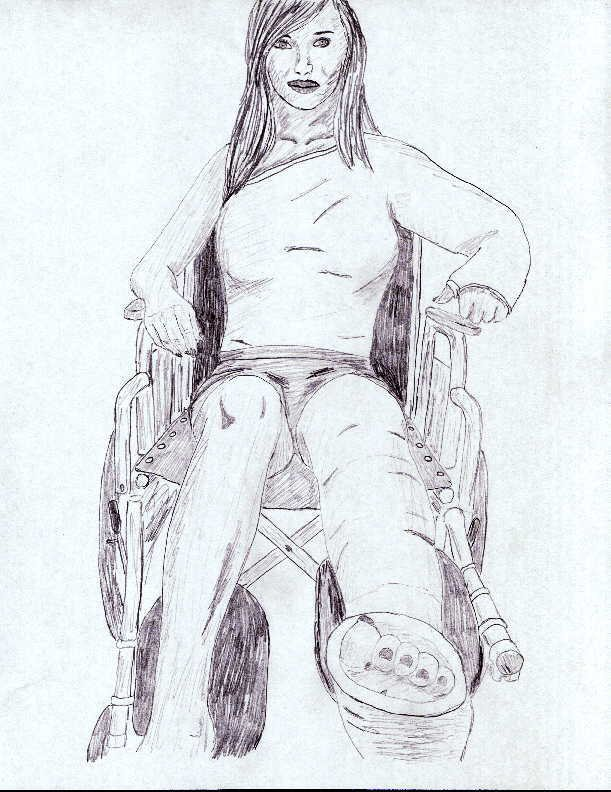
\includegraphics{images/kicks28.jpg}
\end{center}
